\subsection{Конфигурация микроконтроллера}
Конфигурация микроконтроллера является важным этапом его подготовки к работе. Для корректной работы микроконтроллера необходимо произвести настройку периферии. К ней относится:
\begin{itemize}
    \item Источник тактирования
    \item Делители частоты
    \item Порта ввода-вывода общего назначения
    \item Интерфейс отладки
    \item Дополнительные интерфейсы
\end{itemize}
Для конфигурации микроконтроллера STM32 будет использоваться среда разработки STM32CubeMX. Эта среда разработки является бесплатной и поддерживает широкий набор микроконтроллеров STM32. Кроме того, она имеет простой и интуитивно понятный интерфейс, что делает её удобной для начинающих разработчиков.

Использование STM32CubeMX для конфигурации микроконтроллера STM32 позволяет значительно упростить и ускорить этот процесс. Среда разработки предоставляет графический интерфейс, который позволяет легко и быстро настроить все необходимые параметры периферии.

\subsubsection{Конфигурация тактирования}
Конфигурация тактирования позволяет выбрать источник тактовой частоты микроконтроллера, а также настроить частоту и режим работы генератора. Она также позволяет настроить делители частоты, которые используются для получения тактовых частот для различных модулей микроконтроллера.
\begin{figure}[h!]
    \centering
    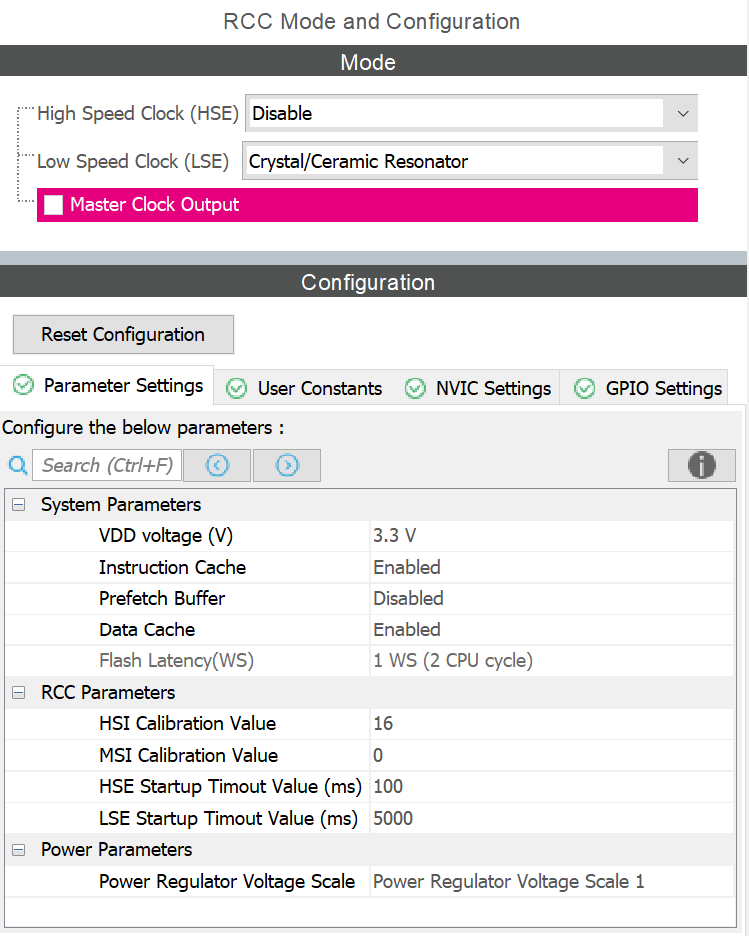
\includegraphics[width=0.6\linewidth]{\commonSecPathPrefix/sec_6/content/cube_rcc.png}
    \caption{Конфигурация RCC в STM32CubeMX}
\end{figure}

\subsubsection{Конфигурация портов ввода-вывода}
Конфигурация портов ввода-вывода позволяет настроить назначение выводов портов микроконтроллера, а также настроить режим работы вывода, его параметры ввода/вывода и другие свойства.
\begin{figure}[h!]
    \centering
    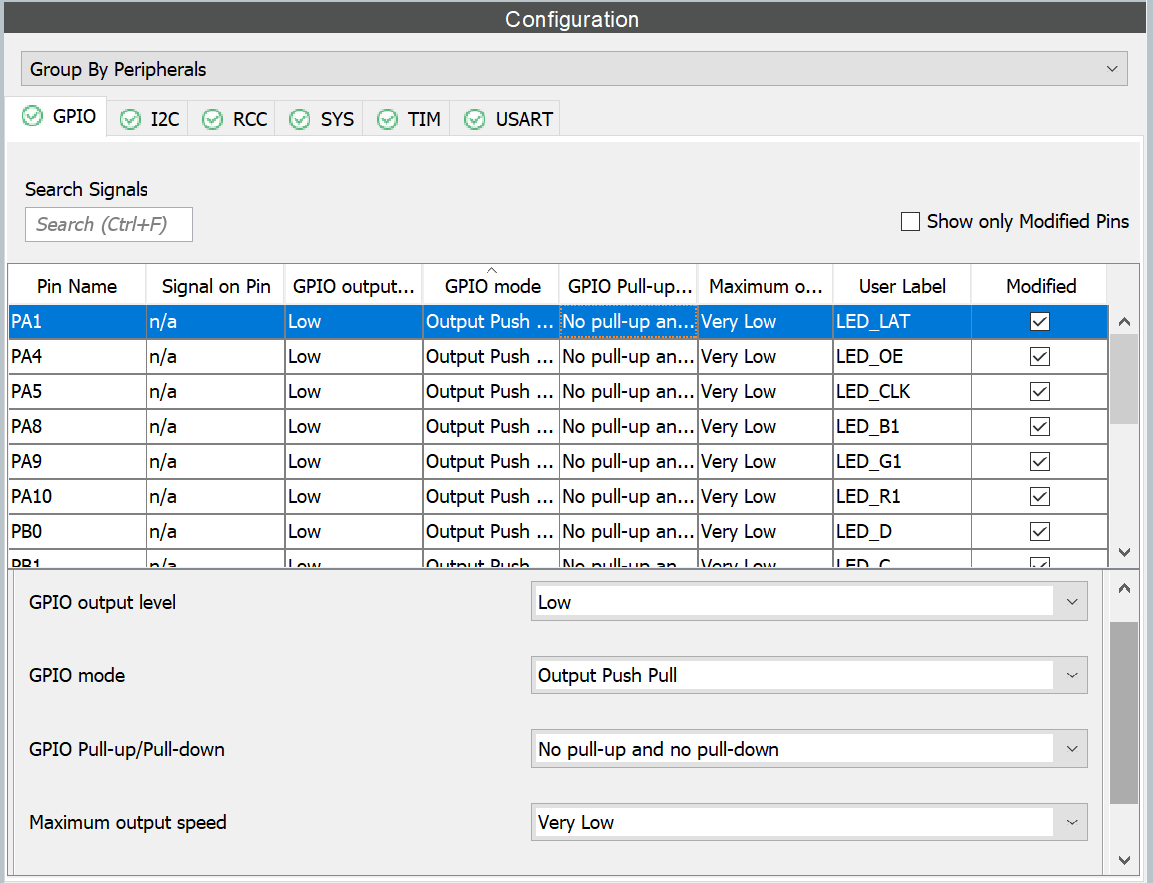
\includegraphics[width=0.6\linewidth]{\commonSecPathPrefix/sec_6/content/cube_gpio.png}
    \caption{Конфигурация портов GPIO в STM32CubeMX}
\end{figure}

\subsubsection{Конфигурация интерфейса отладки}
Конфигурация интерфейса отладки позволяет настроить интерфейс отладки микроконтроллера, а также настроить параметры интерфейса, такие как скорость передачи данных и режим работы. 
\begin{figure}[h!]
    \centering
    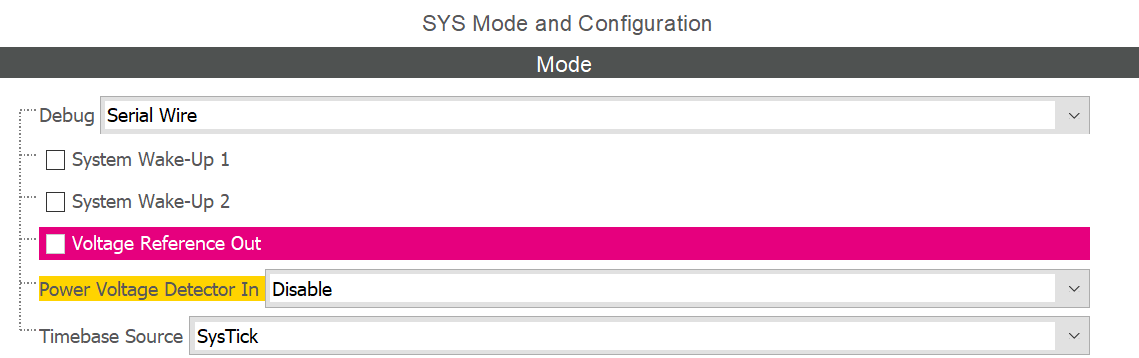
\includegraphics[width=0.6\linewidth]{\commonSecPathPrefix/sec_6/content/cube_swd.png}
    \caption{Конфигурация отладки SWD в STM32CubeMX}
\end{figure}

\subsubsection{Конфигурация дополнительных интерфейсов}
Конфигурация дополнительных интерфейсов позволяет настроить дополнительные интерфейсы микроконтроллера, такие как USB, USART, SPI и I2C. Для каждого интерфейса можно настроить параметры, такие как частота, режим работы и другие свойства.
\begin{figure}[h!]
    \centering
    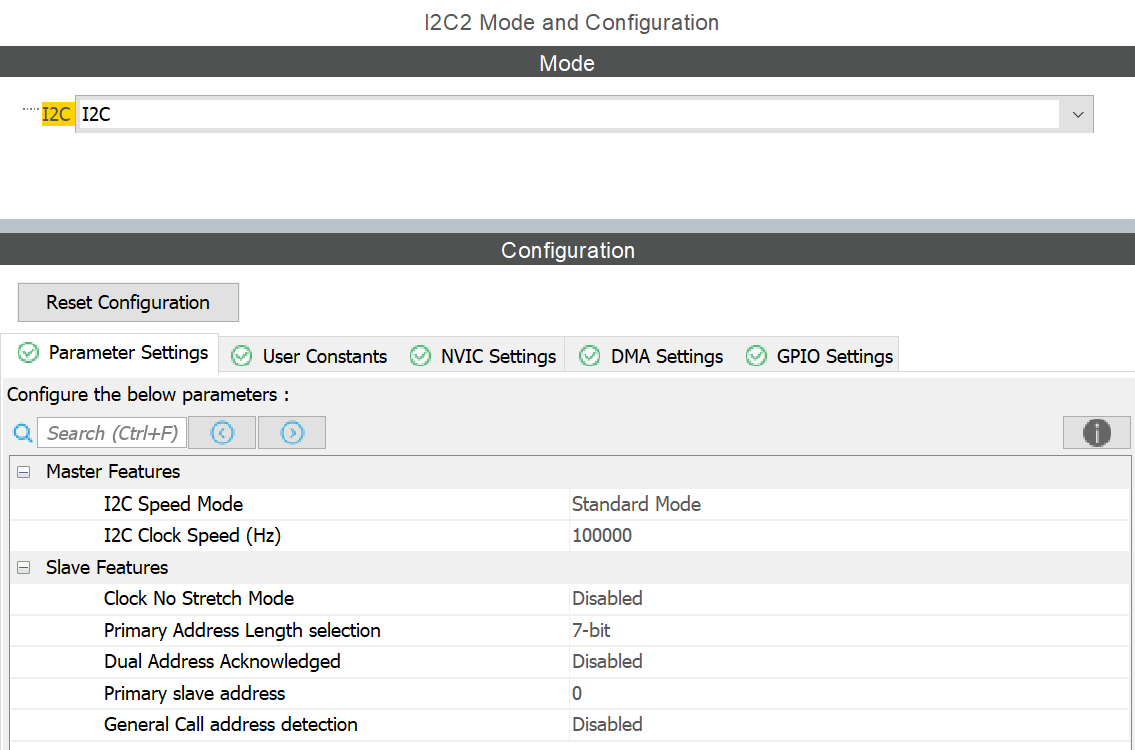
\includegraphics[width=0.6\linewidth]{\commonSecPathPrefix/sec_6/content/cube_i2c.png}
    \caption{Конфигурация I2C в STM32CubeMX}
\end{figure}
\begin{figure}[h!]
    \centering
    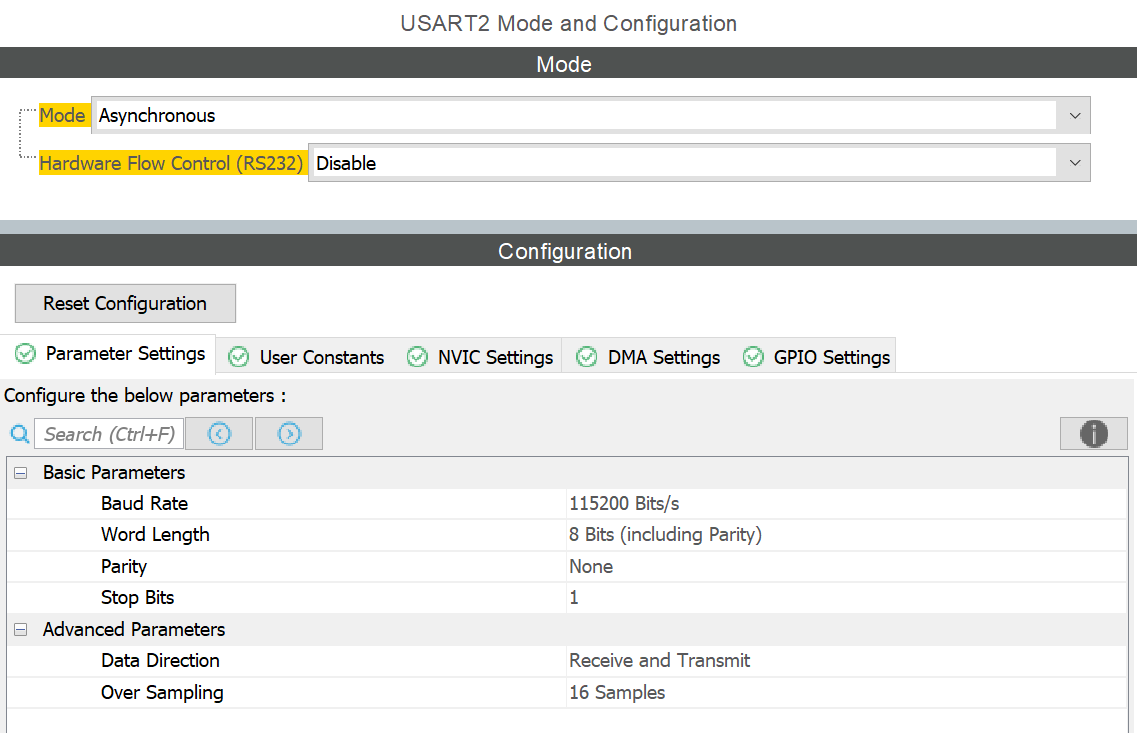
\includegraphics[width=0.6\linewidth]{\commonSecPathPrefix/sec_6/content/cube_usart.png}
    \caption{Конфигурация USART в STM32CubeMX}
\end{figure}